\documentclass[aspectratio=169]{beamer}

\usepackage{fontspec}
\usepackage{microtype}
\usepackage{fontawesome}
\usepackage{emoji}
\usepackage{tikz}
\usetikzlibrary{positioning, calc, patterns}
\usetikzlibrary{overlay-beamer-styles}
\setbeamertemplate{frametitle}[default][center]

\hypersetup{
    colorlinks,
    linkcolor=red,
    pdftitle={What is a range?},
    pdfpagemode=FullScreen,
    }

\setmonofont{JetBrainsMonoNL}[
    Path=./static/fonts/jetbrains/,
    Scale=0.85,
    Extension = .ttf,
    UprightFont=*-Regular,
    BoldFont=*-Bold,
    ItalicFont=*-Italic,
    BoldItalicFont=*-BoldItalic
    ]
    
\setsansfont{Asap}[
    Path=./static/fonts/asap/,
    Scale=0.9,
    Extension = .ttf,
    UprightFont=*-Regular,
    BoldFont=*-Bold,
    ItalicFont=*-Italic,
    BoldItalicFont=*-BoldItalic
    ]
    
\usepackage[newfloat=true]{minted}
%\usemintedstyle{xcode}
\beamertemplatenavigationsymbolsempty

\setbeamertemplate{footline}{\begin{center}\quad\insertframenumber\strut\quad\end{center}}
\setbeamerfont{footline}{size=\large}

\date{July 4, 2024}

%\setbeameroption{hide notes} % Only slides
%\setbeameroption{show only notes} % Only notes
%\setbeameroption{show notes on second screen=left}

\title{What is a range?}
\author{Šimon Tóth}

\begin{document}

{\usebackgroundtemplate{%
  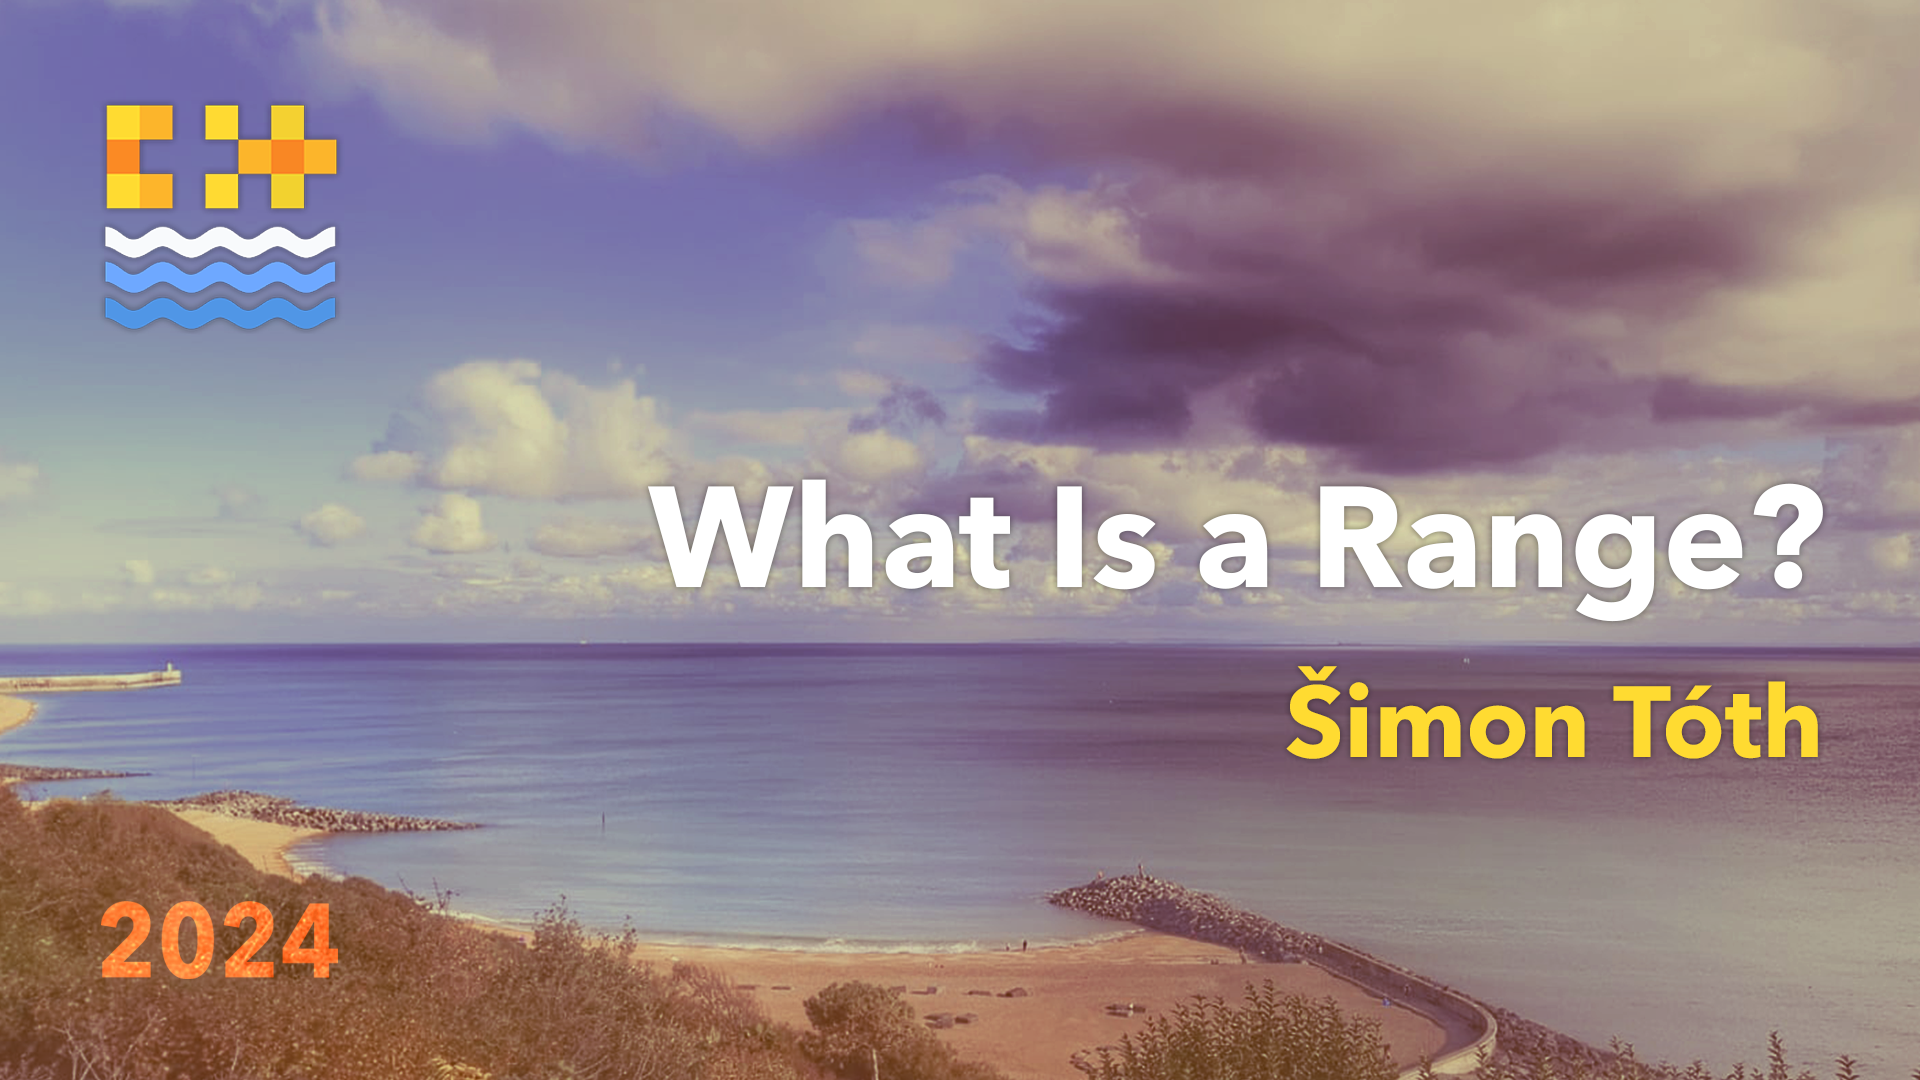
\includegraphics[width=\paperwidth,height=\paperheight]{static/cpp-on-sea-title.png}} 
\begin{frame}
\end{frame}}

\begin{frame}{Slides}
\Large
\begin{center}
    \url{https://github.com/HappyCerberus/what-is-a-range}
    
\includegraphics[height=.7\textheight]{static/qrcode.png}
\end{center}
\end{frame}

\begin{frame}[c]
    \Huge
    \begin{center}
        Ask questions!
    \end{center}
\end{frame}

\begin{frame}{A Complete Guide to Standard C++ Algorithms}
\begin{columns}
    \begin{column}{0.35\textwidth}
        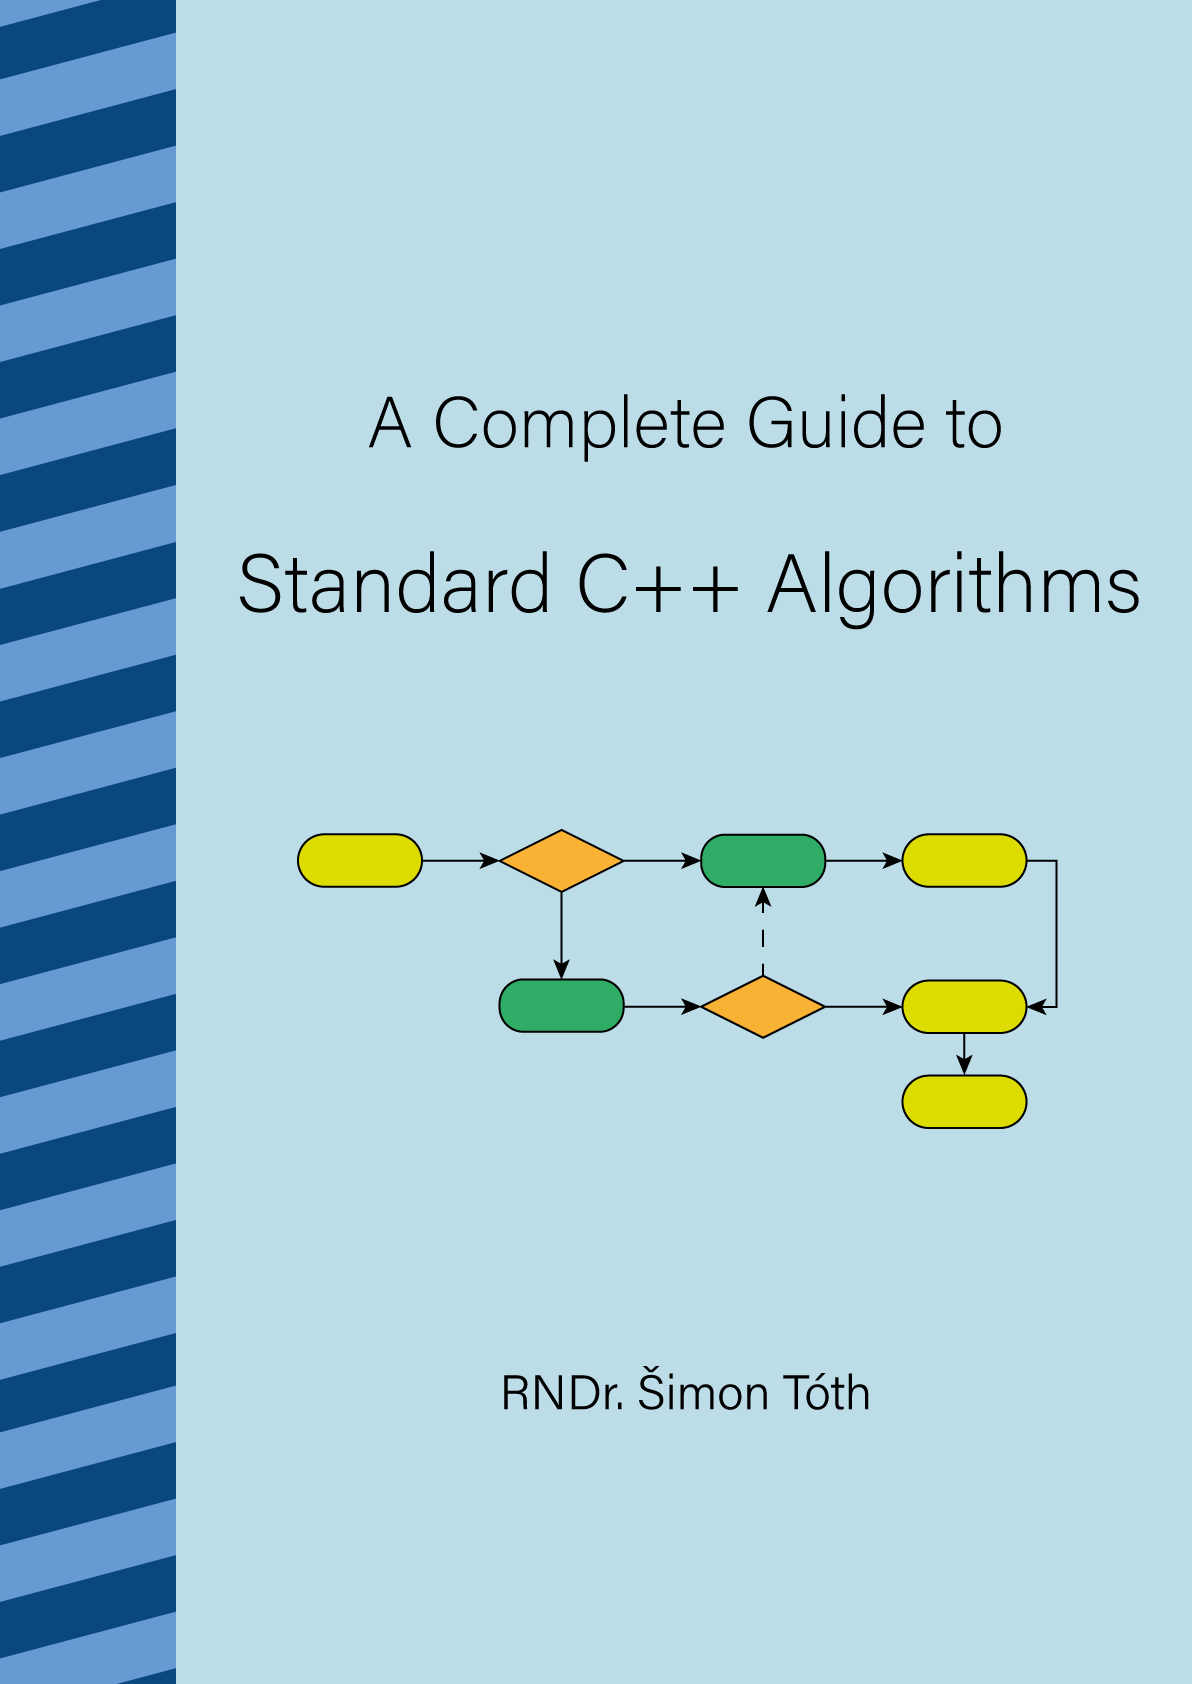
\includegraphics[height=0.8\textheight]{static/book_algorithms.png}
    \end{column}
    \begin{column}{0.6\textwidth}
        \begin{itemize}
            \item Content complete for C++20
            \item Free on GitHub:\\
                \href{https://github.com/HappyCerberus/book-cpp-algorithms}{HappyCerberus/book-cpp-algorithms}
            \item Donate to EFF on LeanPub:\\
                \href{https://leanpub.com/cpp-algorithms-guide}{leanpub.com/cpp-algorithms-guide}
        \end{itemize}
    \end{column}
\end{columns}
\end{frame}

\begin{frame}{Surviving the C++ Coding Interview}
\begin{columns}
    \begin{column}{0.35\textwidth}
        
\includegraphics[height=0.8\textheight]{static/book_interview.png}
    \end{column}
    \begin{column}{0.6\textwidth}
        \begin{itemize}
            \item Work in progress (95 pages)
            \item Free Community Edition:\\
                \href{https://leanpub.com/cpp-coding-interview/signup}{leanpub.com/cpp-coding-interview/signup}
            \item Donate to EFF on LeanPub:\\
                \href{https://leanpub.com/cpp-coding-interview}{leanpub.com/cpp-coding-interview}
        \end{itemize}
    \end{column}
\end{columns}
\end{frame}

\begin{frame}{Daily bit(e) of C++}
\begin{columns}
    \begin{column}{0.35\textwidth}
        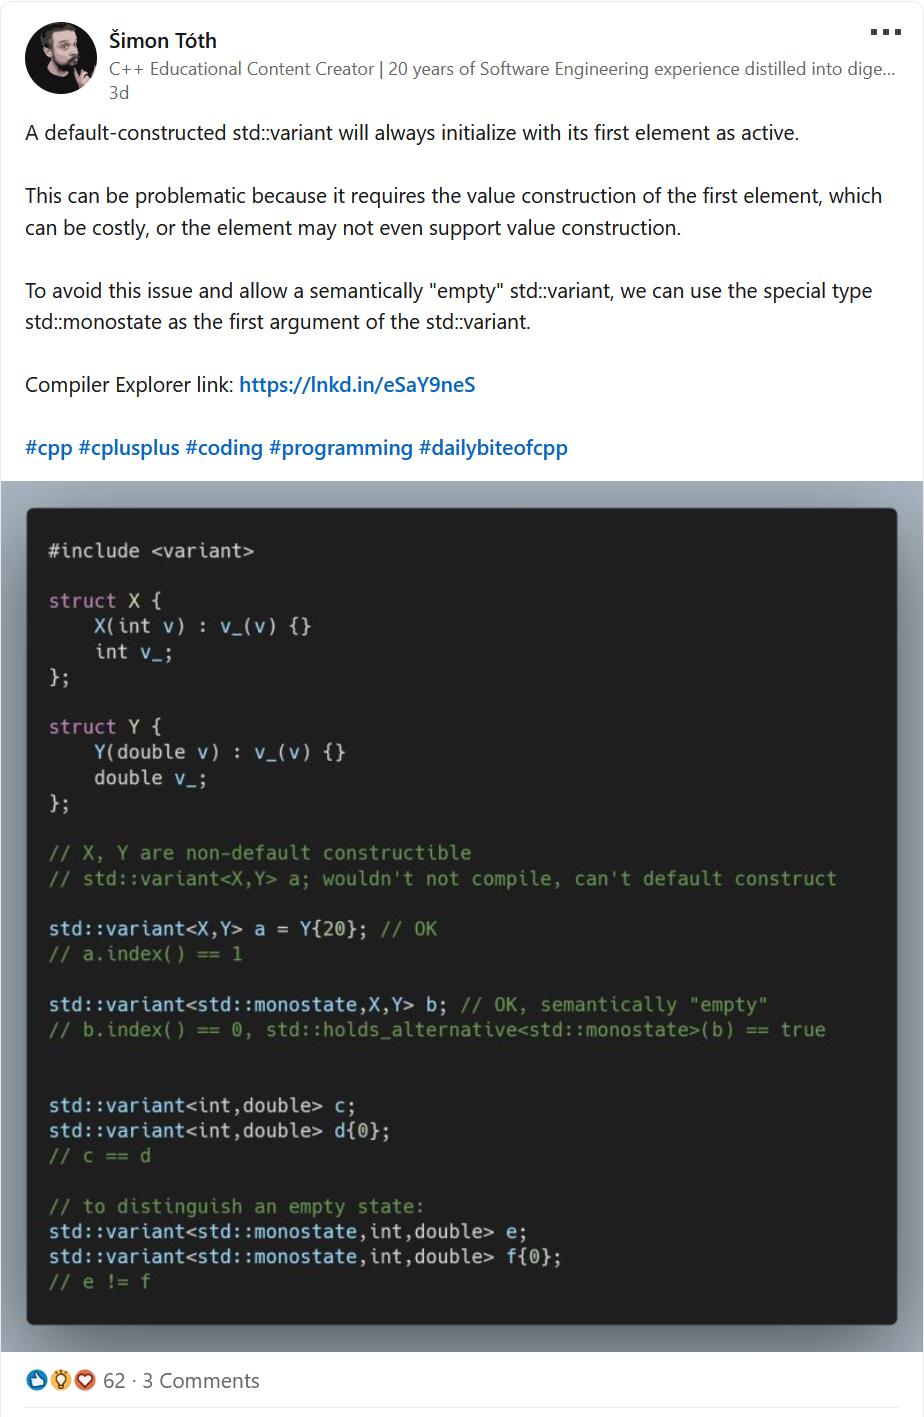
\includegraphics[height=0.8\textheight]{static/daily_bite.png}
    \end{column}
    \begin{column}{0.6\textwidth}
        \begin{itemize}
            \item \href{https://www.linkedin.com/in/simontoth/}{linkedin.com/in/simontoth}
            \item \href{https://hachyderm.io/@simontoth}{hachyderm.io/@simontoth}
            \item \href{https://medium.com/@simontoth}{medium.com/@simontoth}
            \item \href{https://simontoth.substack.com}{simontoth.substack.com}
            \item \href{https://github.com/HappyCerberus/daily-bite-cpp}{github.com/HappyCerberus/daily-bite-cpp}
        \end{itemize}
    \end{column}
\end{columns}
\end{frame}

% Timecheck 03:30 / 03:30

\begin{frame}[c]
    \Huge
    \begin{center}
        What is a range? (pre-C++20)
    \end{center}
\end{frame}

\begin{frame}[fragile,c]
\Large
\begin{center}
\begin{minted}[escapeinside=||]{cpp}
auto first = container.begin();
auto last = container.end();

|\pause|using std::begin; 
auto first = begin(container);
using std::end;
auto last = end(container);
\end{minted}
\end{center}
\end{frame}

\begin{frame}[fragile,c]
\Large
\begin{center}
\begin{minted}[escapeinside=||]{cpp}
struct Member {
    struct Iterator {};
    Iterator begin() { return {}; }
};

using std::begin;

Member m;
auto it = begin(m);
// decltype(it) == Member::Iterator
\end{minted}
\end{center}
\let\thefootnote\relax\footnotetext{\url{https://compiler-explorer.com/z/qnTxYcr7z}}
\end{frame}

\begin{frame}[fragile,c]
\Large
\begin{center}
\begin{minted}[escapeinside=||]{cpp}
int arr[5];

using std::begin;

auto it = begin(arr);
// it == arr
// decltype(it) == int*
\end{minted}
\end{center}
\let\thefootnote\relax\footnotetext{\url{https://compiler-explorer.com/z/qnTxYcr7z}}
\end{frame}

\begin{frame}[fragile,c]
\Large
\begin{center}
\begin{minted}[escapeinside=||]{cpp}
struct Friend {
    struct Iterator {};
    friend Iterator begin(const Friend&) { return {}; }
};

using std::begin;

Friend f;
auto it = begin(f);
// decltype(it) == Friend::Iterator
\end{minted}
\end{center}
\let\thefootnote\relax\footnotetext{\url{https://compiler-explorer.com/z/qnTxYcr7z}}
\end{frame}

\begin{frame}[fragile,c]
\Large
\begin{center}
\begin{minted}[escapeinside=||]{cpp}
auto first = container.begin();
auto last = container.end();

for (auto it = first; it != last; ++it)
    std::println("{}", *it);
\end{minted}
\end{center}
\end{frame}

\tikzstyle{element} = [rectangle, draw=red!60, fill=red!5, thick, minimum size=2cm, text depth=.0\baselineskip, text height=.7\baselineskip]
\tikzstyle{empty} = [rectangle, draw=black!60, fill=black!5, thick, minimum size=2cm, text depth=.0\baselineskip, text height=.7\baselineskip]

\begin{frame}
    \begin{tikzpicture}[overlay, remember picture]
        \node[element](center) at (current page.center){};
        \node[element](l1)[left=0cm of center]{};
        \node[element](l2)[left=0cm of l1]{};
        \node[element](r1)[right=0cm of center]{};
        \node[empty](r2)[right=0cm of r1]{};
        \node(begin)[below=1cm of l2]{\Large{begin}};
        \node(end)[below=1cm of r2]{\Large{end}};
        \draw[thick, ->](begin)--(l2);
        \draw[thick, ->](end)--(r2);
    \end{tikzpicture}
\end{frame}

\begin{frame}
    \begin{tikzpicture}[overlay, remember picture]
        \node[empty](center) at (current page.center){};
        \node(begin)[below=1cm of center.south west]{\Large{begin}};
        \node(end)[below=1cm of center.south east]{\Large{end}};
        \draw[thick, ->, transform canvas={xshift=1em}](begin)--(center.south west);
        \draw[thick, ->, transform canvas={xshift=-1em}](end)--(center.south east);
    \end{tikzpicture}
\end{frame}

\begin{frame}
    \begin{tikzpicture}[overlay, remember picture]
        \node[element](center) at (current page.center){};
        \node[element](l1)[left=0cm of center]{};
        \node[element](l2)[left=0cm of l1]{};
        \node[element](r1)[right=0cm of center]{};
        \node[empty](r2)[right=0cm of r1]{};
        \node(begin)[below=1cm of l2]{\Large{begin}};
        \node(end)[below=1cm of r2]{\Large{end}};
        \node(mid)[below=1cm of center]{\Large{mid}};
        \draw[thick, ->](begin)--(l2);
        \draw[thick, ->](end)--(r2);
        \draw[thick, ->](mid)--(center);
    \end{tikzpicture}
\end{frame}

\begin{frame}
    \begin{tikzpicture}[overlay, remember picture]
        \node[element](center) at ([xshift=2cm]current page.center){};
        \node[empty](l1)[left=2cm of center]{};
        \node[element](l2)[left=0cm of l1]{};
        \node[element](l3)[left=0cm of l2]{};
        \node[element](r1)[right=0cm of center]{};
        \node[empty](r2)[right=0cm of r1]{};
        \node(begin)[below=1cm of l3]{\Large{begin}};
        \node(end)[below=1cm of r2]{\Large{end}};
        \node(mid)[below=1cm of center]{\Large{mid}};
        \node(midn)[below=1cm of l1]{\Large{mid}};
        \draw[thick, ->](begin)--(l3);
        \draw[thick, ->](end)--(r2);
        \draw[thick, ->](mid)--(center);
        \draw[thick, ->](midn)--(l1);
    \end{tikzpicture}
\end{frame}

\begin{frame}[fragile,c]
\Huge
\begin{center}
\begin{minted}[escapeinside=||]{cpp}
[first, last)
\end{minted}
\end{center}
\end{frame}

\begin{frame}[fragile,c]
\Huge
\begin{center}
\begin{minted}[escapeinside=||]{cpp}
{0, 1, 2, 3, 4, 5, 6, 7, 8, 9}
[0, 10)
\end{minted}
\end{center}
\end{frame}

\begin{frame}[fragile,c]{}
\Large
\begin{center}
\begin{minted}[escapeinside=||]{cpp}
int data[5] = {1,2,3,4,5};

|\pause|int* first = data;
int* last = first + 5; // one past

|\pause|for (int* it = first; it != last; ++it)
    std::println("{}", *it);
\end{minted}
\end{center}
\let\thefootnote\relax\footnotetext{\url{https://compiler-explorer.com/z/89d5f6h7b}}
\end{frame}

\begin{frame}[fragile,c]{}
\Large
\begin{center}
\begin{minted}[escapeinside=||]{cpp}
List list = {1,2,3,4,5};

Node* first = list.head();
Node* last = nullptr;

for (Node* it = first; it != last; it = it->next)
    std::println("{}", it->value);
\end{minted}
\end{center}
\let\thefootnote\relax\footnotetext{\url{https://compiler-explorer.com/z/5Ecdhqaa4}}
\end{frame}

\begin{frame}[fragile,c]{}
\Large
\begin{center}
\begin{minted}[escapeinside=||]{cpp}
for (int* it = first; it != last; ++it)
    std::println("{}", *it);

for (Node* it = first; it != last; it = it->next)
    std::println("{}", it->value);
\end{minted}
\end{center}
\end{frame}

\begin{frame}[fragile,c]{}
\Large
\begin{center}
\begin{minted}[escapeinside=||]{cpp}
std::forward_list<int> list{1,2,3,4,5};

auto first = list.begin();
auto last = list.end();

for (auto it = first; it != last; ++it)
    std::println("{}", *it);
\end{minted}
\end{center}
\let\thefootnote\relax\footnotetext{\url{https://compiler-explorer.com/z/jrP9GeG5e}}
\end{frame}

\begin{frame}[fragile]{input/output}
    \begin{itemize}
        \item \mintinline{cpp}{std::istream_iterator}, \mintinline{cpp}{std::ostream_iterator}
    \end{itemize}
    \begin{itemize}
        \item \emph{base:} \mintinline{cpp}{*it}, \mintinline{cpp}{++it}, \mintinline{cpp}{it++}
    \end{itemize}
\end{frame}

\begin{frame}[fragile]{forward}
    \begin{itemize}
        \item \mintinline{cpp}{std::forward_list}
    \end{itemize}
    \begin{itemize}
        \item base: \mintinline{cpp}{*it}, \mintinline{cpp}{++it}, \mintinline{cpp}{it++}
        \item \emph{multi-access:} \mintinline{cpp}{auto it2 = it1; ++it1; *it1; *it2;}
    \end{itemize}
\end{frame}

\begin{frame}[fragile]{bidirectional}
    \begin{itemize}
        \item \mintinline{cpp}{std::set}, \mintinline{cpp}{std::map}
    \end{itemize}
    \begin{itemize}
        \item base: \mintinline{cpp}{*it}, \mintinline{cpp}{++it}, \mintinline{cpp}{it++}
        \item multi-access: \mintinline{cpp}{auto it2 = it1; ++it1; *it1; *it2;}
        \item \emph{bidirectional:} \mintinline{cpp}{--it}, \mintinline{cpp}{it--}
    \end{itemize}
\end{frame}

\begin{frame}[fragile]{random access}
    \begin{itemize}
        \item \mintinline{cpp}{std::deque}
    \end{itemize}
    \begin{itemize}
        \item base: \mintinline{cpp}{*it}, \mintinline{cpp}{++it}, \mintinline{cpp}{it++}
        \item multi-access: \mintinline{cpp}{auto it2 = it1; ++it1; *it1; *it2;}
        \item bidirectional: \mintinline{cpp}{--it}, \mintinline{cpp}{it--}
        \item \emph{random access:} \mintinline{cpp}{it + offset}, \mintinline{cpp}{it - offset}
        \item \emph{distance:} \mintinline{cpp}{it1 - it2}
    \end{itemize}
\end{frame}

\begin{frame}[fragile]{contiguous}
\begin{itemize}
    \item \mintinline{cpp}{std::array}, \mintinline{cpp}{std::vector}
\end{itemize}
\begin{itemize}
    \item base: \mintinline{cpp}{*it}, \mintinline{cpp}{++it}, \mintinline{cpp}{it++}
    \item multi-access: \mintinline{cpp}{auto it2 = it1; ++it1; *it1; *it2;}
    \item bidirectional: \mintinline{cpp}{--it}, \mintinline{cpp}{it--}
    \item random access: \mintinline{cpp}{it + offset}, \mintinline{cpp}{it - offset}
    \item distance: \mintinline{cpp}{it1 - it2}
    \item \emph{contiguous memory}
\end{itemize}
\end{frame}

% Timecheck 08:30 / 12:00

\begin{frame}[c]
    \Huge
    \begin{center}
        What is a range?
    \end{center}
\end{frame}

\begin{frame}[fragile,c]
    \Large
    \begin{itemize}
        \item \mintinline{cpp}{for (auto e : rng) {}}
        \pause \item \mintinline{cpp}{begin(rng)}, \mintinline{cpp}{end(rng)}
        \pause \item input or output iterator
        \pause \item \mintinline{cpp}{[begin(rng), end(rng))}
    \end{itemize}
\end{frame}

\begin{frame}[fragile,c]
\Large
\begin{center}
\begin{minted}[escapeinside=||]{cpp}
namespace std::ranges {
    template<class T>
    concept range = requires(T& t) {
        ranges::begin(t);
        ranges::end  (t);
    };
}
\end{minted}
\end{center}
\end{frame}

\begin{frame}[fragile,c]
\Large
\begin{center}
\begin{minted}[escapeinside=||]{cpp}
int arr[5] = {1,2,3,4,5};

auto first = std::ranges::begin(arr);
auto last = std::ranges::end(arr);

for (auto it = first; it != last; ++it)
    std::println("{}", *it);
\end{minted}
\end{center}
\let\thefootnote\relax\footnotetext{\url{https://compiler-explorer.com/z/b67PnGWP8}}
\end{frame}

\begin{frame}[fragile,c]
\Large
\begin{center}
\begin{minted}[escapeinside=||]{cpp}
int arr[5] = {1,2,3,4,5};

auto first = std::ranges::begin(arr);
auto last = std::ranges::end(arr);

for (auto& e : std::ranges::subrange(first, last))
    std::println("{}", e);
\end{minted}
\end{center}
\let\thefootnote\relax\footnotetext{\url{https://compiler-explorer.com/z/dMozG7j8h}}
\end{frame}

 \begin{frame}{Range concepts}
    \begin{itemize}
        \item \mintinline{cpp}{ranges::input_range}
        \item \mintinline{cpp}{ranges::output_range}
        \item \mintinline{cpp}{ranges::forward_range}
        \item \mintinline{cpp}{ranges::bidirectional_range}
        \item \mintinline{cpp}{ranges::random_access_range}
        \item \mintinline{cpp}{ranges::contiguous_range}
    \end{itemize}
\end{frame}

\begin{frame}[fragile,c]
\large
\begin{center}
\begin{minted}[escapeinside=||]{cpp}
auto sum(std::ranges::input_range auto&& rng) {
    auto result = std::ranges::range_value_t<decltype(rng)>{};
    for (auto& e : rng)
        result += e;
    return result;
}
\end{minted}
\end{center}
\let\thefootnote\relax\footnotetext{\url{https://compiler-explorer.com/z/f5h7jYnjP}}
\end{frame}

\begin{frame}[fragile,c]
\large
\begin{center}
\begin{minted}[escapeinside=||]{cpp}
template <std::ranges::input_range Rng>
auto sum(Rng&& rng) {
    auto result = std::ranges::range_value_t<Rng>{};
    for (auto& e : rng)
        result += e;
    return result;
}
\end{minted}
\end{center}
\let\thefootnote\relax\footnotetext{\url{https://compiler-explorer.com/z/a9qx5rWh1}}
\end{frame}

\begin{frame}[c]
    \Huge
    \begin{center}
        Universal reference
    \end{center}
\end{frame}

% Timestamp 4:00, 16:00

\begin{frame}[fragile,c]
\large
\begin{center}
\begin{minted}[escapeinside=||]{cpp}
const char& find_second(const std::string& str, char c) {
    static char not_found = '\0';

    size_t idx = str.find(c);
    if (idx == std::string::npos) return not_found;

    idx = str.find(c, idx+1);
    if (idx == std::string::npos) return not_found;

    return str[idx];
}

|\pause|const char &c = find_second("Hello World!", 'o');
\end{minted}
\end{center}
\let\thefootnote\relax\footnotetext{\url{https://compiler-explorer.com/z/E6EqjzTKr}}
\end{frame}

\begin{frame}[fragile,c]
\large
\begin{center}
    \begin{minted}[escapeinside=||]{cpp}
const char& find_second(const std::string_view& str, char c) {
    static char not_found = '\0';

    size_t idx = str.find(c);
    if (idx == std::string::npos) return not_found;

    idx = str.find(c, idx+1);
    if (idx == std::string::npos) return not_found;

    return str[idx];
}

const char &c = find_second("Hello World!", 'o');
    \end{minted}
\end{center}
\let\thefootnote\relax\footnotetext{\url{https://compiler-explorer.com/z/79Wej378n}}
\end{frame}

\begin{frame}{Borrowed range}
    \begin{itemize}
        \item \mintinline{cpp}{std::string_view}
        \item \mintinline{cpp}{std::span}
    \end{itemize}
\end{frame}

\begin{frame}[fragile,c]{Range algorithms}
\begin{center}
\begin{minted}[escapeinside=||]{cpp}
auto it1 = std::ranges::find(std::string_view("Hello World!"), 'o');
// decltype(it1) == std::string_view::iterator
// *it1 == 'o'

|\pause|auto it2 = std::ranges::find(std::string("Hello World!"), 'o');
// decltype(it2) == std::ranges::dangling

|\pause|std::string str1("Hello World!");
auto it3 = std::ranges::find(str1, 'o');
// decltype(it3) == std::string::iterator

std::string_view str2("Hello World!");
auto it4 = std::ranges::find(str2, 'o');
// decltype(it4) == std::string_view::iterator
\end{minted}
\end{center}
\let\thefootnote\relax\footnotetext{\url{https://compiler-explorer.com/z/E5cMG4qqT}}
\end{frame}

\begin{frame}[fragile]
\begin{center}
\begin{minted}[escapeinside=||]{cpp}
void fun(const std::string& rng) {}

fun(std::string("")); // taking ownership

std::string str;
fun(str);             // borrowing
\end{minted}
\end{center}
\end{frame}

\begin{frame}[fragile]
\begin{center}
\begin{minted}[escapeinside=||]{cpp}
void fun(auto&& rng) {
    if constexpr (std::ranges::borrowed_range<decltype(rng)>) {
        // borrowing
    } else {
        // taking ownership
    }
}

fun(std::string(""));      // taking ownership
fun(std::string_view("")); // borrowing

std::string str;
fun(str);                  // borrowing
fun(std::as_const(str));   // borrowing
\end{minted}
\end{center}
\let\thefootnote\relax\footnotetext{\url{https://compiler-explorer.com/z/h436jzTaq}}
\end{frame}

\begin{frame}[fragile]
\begin{minted}[escapeinside=||]{cpp}
template <std::ranges::forward_range Str>
requires std::ranges::borrowed_range<Str> 
    && std::same_as<std::ranges::range_value_t<Str>,char>
const char& find_second(Str&& str, char c) {
    /* ... */
}
\end{minted}
\let\thefootnote\relax\footnotetext{\url{https://compiler-explorer.com/z/x68W8PGEq}}
\end{frame}

\begin{frame}[fragile,c]
    \large
    \begin{center}
        \begin{minted}[escapeinside=||]{cpp}
template <std::ranges::input_range Rng>
auto sum(Rng&& rng) {
    auto result = std::ranges::range_value_t<Rng>{};
    for (auto& e : rng)
        result += e;
    return result;
}
        \end{minted}
    \end{center}
\end{frame}

% Time 7:00, 23:00

\begin{frame}[c]
    \Huge
    \begin{center}
        Views
    \end{center}
\end{frame}

{\usebackgroundtemplate{%
  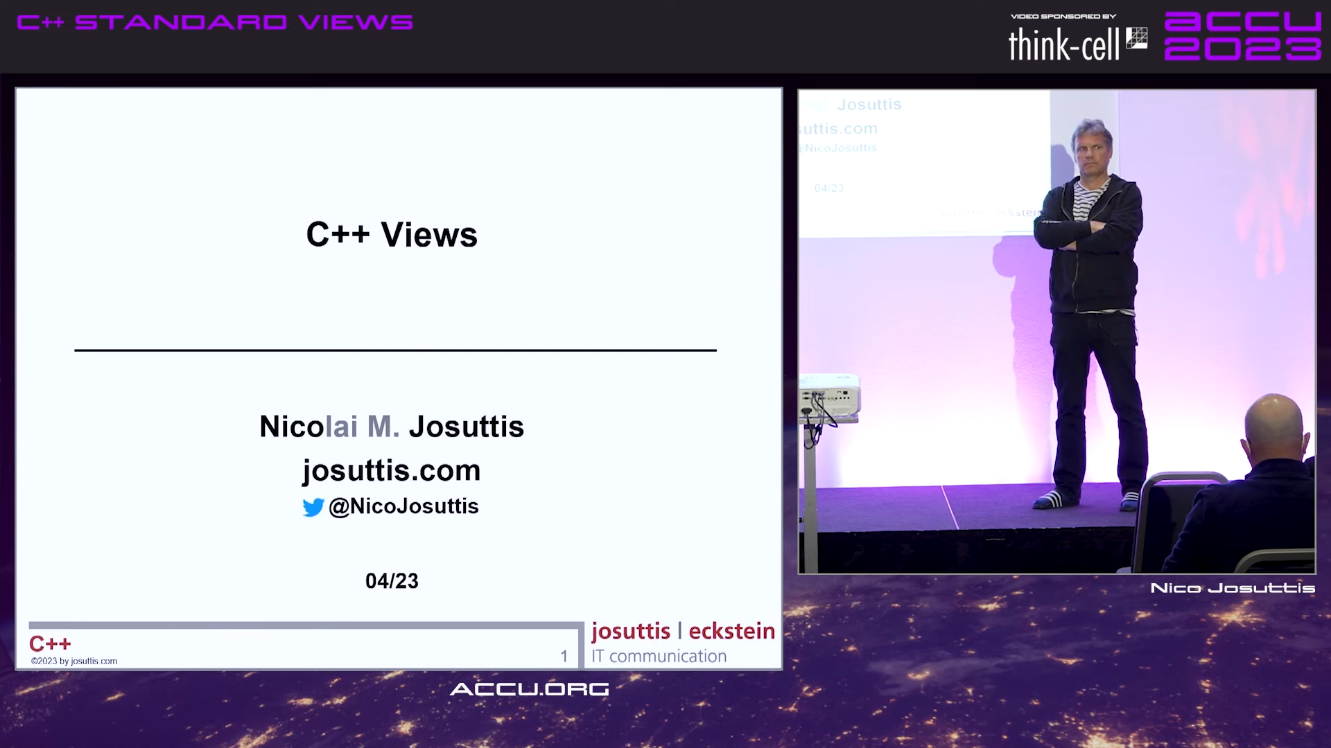
\includegraphics[width=\paperwidth,height=\paperheight]{static/nico_talk.png}} 
\begin{frame}
\end{frame}}

\begin{frame}{View}
    \begin{itemize}
        \item cheap to move
        \item cheap to destroy when moved-from
        \item cheap to copy if copyable
    \end{itemize}
\end{frame}

\begin{frame}[fragile,c]{Not a borrowed range}
\large
\begin{center}
\begin{minted}[escapeinside=||]{cpp}
std::vector<int> data{1,2,3,4,5};
auto rng1 = std::views::all(data);
// borrowed, decltype(rng1) == std::ranges::ref_view<...>

auto rng2 = std::views::all(std::vector<int>{1,2,3,4,5});
// not borrowed, decltype(rng2) == std::ranges::owning_view<...>
\end{minted}
\end{center}
\let\thefootnote\relax\footnotetext{\url{https://compiler-explorer.com/z/T74ffK1dz}}
\end{frame}

\begin{frame}[fragile,c]{Views as code}
\begin{center}
\begin{minted}[escapeinside=!!]{cpp}
std::vector<int> data{1,2,3,4,5};

auto view = data | 
    std::views::transform([](int v) { return v * 2; }) |
    std::views::transform([](int v) { return v + 1; });
// view == {3, 5, 7, 9, 11}
\end{minted}
\end{center}
\let\thefootnote\relax\footnotetext{\url{https://compiler-explorer.com/z/vWE9hq7Mq}}
\end{frame}

\begin{frame}[fragile,c]{Views as code}
\begin{center}
\begin{minted}[escapeinside=!!]{cpp}
std::vector<int> data{1,2,3,4,5};

auto view = data | 
    std::views::transform([](int v) { return v * 2; }) |
    std::views::transform([](int v) { return v + 1; });
// view == {3, 5, 7, 9, 11}

auto manifested = view |
    std::ranges::to<std::vector>();
// decltype(manifested) == std::vector<int>
// manifested == {3, 5, 7, 9, 11}
\end{minted}
\end{center}
\let\thefootnote\relax\footnotetext{\url{https://compiler-explorer.com/z/6Ejjz8b7Y}}
\end{frame}

\begin{frame}[fragile,c]{Views as code}
\begin{center}
\begin{minted}[escapeinside=!!]{cpp}
std::vector<int> data{1,2,3,4,5};

auto view = data | 
    std::views::filter([](int v) { return v % 2 == 0; });
// view == {2, 4}
\end{minted}
\end{center}
\let\thefootnote\relax\footnotetext{\url{https://compiler-explorer.com/z/fbsPc9EYx}}
\end{frame}

\begin{frame}[fragile,c]{Views as code}
\begin{center}
\begin{minted}[escapeinside=!!]{cpp}
std::vector<int> data{1,3,5,7,9};

auto view = data | 
    std::views::filter([](int v) { return v % 2 == 0; });
// view == {}

bool empty = view.begin() == view.end();
// empty == true
\end{minted}
\end{center}
\let\thefootnote\relax\footnotetext{\url{https://compiler-explorer.com/z/j86jKrb5f}}
\end{frame}

\begin{frame}[fragile,c]{Views as code}
\begin{center}
\begin{minted}[escapeinside=!!]{cpp}
std::list<int> data{1,3,5,7,9};

auto view = data | 
    std::views::filter([](int v) { return v % 2 == 0; });
// view == {}

bool empty = view.begin() == view.end();
// empty == true

data.push_front(2);

empty = view.begin() == view.end();
// empty == true
\end{minted}
\end{center}
\let\thefootnote\relax\footnotetext{\url{https://compiler-explorer.com/z/WedM1eE8z}}
\end{frame}

\begin{frame}[fragile,c]{Views as code}
\begin{center}
\begin{minted}[escapeinside=!!]{cpp}
void fn(const auto& rng) {
    auto b = rng.begin();
}

fn(std::vector<int>{1,3,5,7,9} |
    std::views::filter([](int v) { return v % 2 == 0; }));
\end{minted}
\end{center}
\let\thefootnote\relax\footnotetext{\url{https://compiler-explorer.com/z/hzd5Ksezd}}
\end{frame}

\begin{frame}[fragile,c]{Views as code}
\begin{center}
\begin{minted}[escapeinside=!!]{cpp}
void fn(auto&& rng) {
    auto b = rng.begin();
}

fn(std::vector<int>{1,3,5,7,9} |
    std::views::filter([](int v) { return v % 2 == 0; }));
\end{minted}
\end{center}
\let\thefootnote\relax\footnotetext{\url{https://compiler-explorer.com/z/G1Tzf3ePa}}
\end{frame}

\begin{frame}[c]
    \large
    \begin{center}
        When taking a range as an argument, always use a universal reference.
    \end{center}
\end{frame}

\begin{frame}[c]
    \Huge
    \begin{center}
        Input ranges
    \end{center}
\end{frame}

\begin{frame}[fragile,c]{\texttt{std::views::istream}}
\small
\begin{center}
\begin{minted}[escapeinside=!!]{cpp}
// standard input: 1 2 3 4 5 6 7 8 9

!\pause!std::vector<int> out1;
std::ranges::copy(
    std::views::istream<int>(std::cin) | std::views::take(3),
    std::back_inserter(out1)
);

std::vector<int> out2;
std::ranges::copy(
    std::views::istream<int>(std::cin) | std::views::take(3),
    std::back_inserter(out2)
);

!\pause!// out1 == {1, 2, 3}
// out2 == {5, 6, 7}
\end{minted}
\end{center}
\let\thefootnote\relax\footnotetext{\url{https://compiler-explorer.com/z/YGvb57K6P}}
\end{frame}

\begin{frame}
    \begin{tikzpicture}[overlay, remember picture]
        \node[element](center) at ([xshift=-1cm] current page.center){2};
        \node[element](l1)[left=0cm of center]{1};
        \node[element](r1)[right=0cm of center]{3};
        \node[empty](r2)[right=0cm of r1]{4};
        \node(it)[below=1cm of l1]{\Large{it}};
        \node(end)[below=1cm of r2]{\Large{end}};
        \draw[thick, ->](it)--(l1);
        \draw[thick, ->](end)--(r2);
    \end{tikzpicture}
\end{frame}

\begin{frame}
    \begin{tikzpicture}[overlay, remember picture]
        \node[element](center) at ([xshift=-1cm] current page.center){2};
        \node[element](l1)[left=0cm of center]{1};
        \node[element](r1)[right=0cm of center]{3};
        \node[empty](r2)[right=0cm of r1]{4};
        \node(it)[below=1cm of r2.south west]{\Large{it}};
        \node(end)[below=1cm of r2.south east]{\Large{end}};
        \draw[thick, ->, transform canvas={xshift=1em}](it)--(r2.south west);
        \draw[thick, ->, transform canvas={xshift=-1em}](end)--(r2.south east);
    \end{tikzpicture}
\end{frame}

\begin{frame}[fragile,c]{\texttt{std::views::istream}}
\small
\begin{center}
\begin{minted}[escapeinside=!!]{cpp}
// standard input: 1 2 3 4 5 6 7 8 9

std::vector<int> out1;
std::ranges::copy(
    std::views::istream<int>(std::cin) | std::views::take(3),
    std::back_inserter(out1)
);

std::vector<int> out2;
std::ranges::copy(
    std::views::istream<int>(std::cin) | std::views::take(3),
    std::back_inserter(out2)
);

// out1 == {1, 2, 3}
// out2 == {5, 6, 7}
\end{minted}
\end{center}
\let\thefootnote\relax\footnotetext{\url{https://compiler-explorer.com/z/YGvb57K6P}}
\end{frame}

\begin{frame}[fragile,c]{\texttt{std::views::istream}}
\small
\begin{center}
\begin{minted}[escapeinside=!!]{cpp}
// standard input: 1 2 3 4 5 6 7 8 9

std::vector<int> out1;
auto [in, out] = std::ranges::copy(
    std::views::istream<int>(std::cin) | std::views::take(3),
    std::back_inserter(out1)
);
!\pause!// decltype(in) == std::ranges::dangling
\end{minted}
\end{center}
\let\thefootnote\relax\footnotetext{\url{https://compiler-explorer.com/z/8Kvjse9PY}}
\end{frame}

\begin{frame}[fragile,c]{\texttt{std::views::istream}}
\small
\begin{center}
\begin{minted}[escapeinside=!!]{cpp}
// standard input: 1 2 3 4 5 6 7 8 9

auto view = std::views::istream<int>(std::cin) | std::views::take(3);

std::vector<int> out1;
auto [in, out] = std::ranges::copy(
    view,
    std::back_inserter(out1)
);
// out1 == {1,2,3}
// *in == 4
\end{minted}
\end{center}
\let\thefootnote\relax\footnotetext{\url{https://compiler-explorer.com/z/zPdjrvhzx}}
\end{frame}

\begin{frame}[c]
    \Huge
    \begin{center}
        Sized range
    \end{center}
\end{frame}

\begin{frame}[fragile,c]
\large
\begin{center}
\begin{minted}[escapeinside=!!]{cpp}
auto count_to_five = std::views::iota(1) |
    std::views::take(5);

std::vector<int> store;

!\pause!store.reserve(count_to_five.size());!\pause! // Will not compile
std::ranges::copy(count_to_five, std::back_inserter(store));
// std::ranges::sized_range<decltype(count_to_five)> == false
\end{minted}
\end{center}
\let\thefootnote\relax\footnotetext{\url{https://compiler-explorer.com/z/138hEf7bj}}
\end{frame}

\begin{frame}[fragile,c]
\large
\begin{center}
\begin{minted}[escapeinside=!!]{cpp}
auto count_to_five = std::views::iota(1) | 
    std::views::take(5);

auto wrapped = std::ranges::subrange(count_to_five, 5);

std::vector<int> store;

store.reserve(wrapped.size());
std::ranges::copy(wrapped, std::back_inserter(store));
// std::ranges::sized_range<decltype(count_to_five)> == false
// std::ranges::sized_range<decltype(wrapped)> == true
\end{minted}
\end{center}
\let\thefootnote\relax\footnotetext{\url{https://compiler-explorer.com/z/77s55j7qY}}
\end{frame}

\begin{frame}[c]
    \Huge
    \begin{center}
        Common range
    \end{center}
\end{frame}

\begin{frame}[fragile,c]
\Large
\begin{center}
\begin{minted}[escapeinside=||]{cpp}
namespace std::ranges {
    template<class T>
    concept range = requires(T& t) {
        ranges::begin(t);
        ranges::end  (t);
    };
}
\end{minted}
\end{center}
\end{frame}

\begin{frame}[fragile,c]
\Large
\begin{center}
\begin{minted}[escapeinside=||]{cpp}
std::vector<int> data{1,2,3,4,5};
// std::ranges::common_range<decltype(data)> == true

|\pause|auto first = data.begin();
// decltype(first) == std::vector<int>::iterator
auto last = data.end();
// decltype(last) == std::vector<int>::iterator

|\pause|int sum = std::accumulate(first, last, 0);
// OK, sum == 15
\end{minted}
\end{center}
\let\thefootnote\relax\footnotetext{\url{https://compiler-explorer.com/z/86nocb3ra}}
\end{frame}

\begin{frame}[fragile,c]
\Large
\begin{center}
\begin{minted}[escapeinside=!!]{cpp}
auto iota = std::views::iota(1) | 
    std::views::take(5);
// std::ranges::common_range<decltype(iota)> == false

!\pause!auto first = iota.begin();
auto last = iota.end();
// decltype(first) != decltype(last)

// Will not compile
int sum = std::accumulate(first, last, 0);
\end{minted}
\end{center}
\let\thefootnote\relax\footnotetext{\url{https://compiler-explorer.com/z/Yd3qj4515}}
\end{frame}

\begin{frame}[fragile,c]
\Large
\begin{center}
\begin{minted}[escapeinside=!!]{cpp}
auto iota = std::views::iota(1) | 
    std::views::take(5) |
    std::views::common;
// std::ranges::common_range<decltype(iota)> == true

auto first = iota.begin();
auto last = iota.end();
// decltype(first) == decltype(last)

int sum = std::accumulate(first, last, 0);
// OK, sum == 15
\end{minted}
\end{center}
\let\thefootnote\relax\footnotetext{\url{https://compiler-explorer.com/z/7sqGdsPqP}}
\end{frame}

\begin{frame}[fragile,c]
\Large
\begin{center}
\begin{minted}[escapeinside=!!]{cpp}
auto iota = std::views::iota(1) | 
    std::views::take(5);
// std::ranges::common_range<decltype(iota)> == false

int sum = std::ranges::fold_left(iota, 0, std::plus<>{});
// OK, sum == 15
\end{minted}
\end{center}
\let\thefootnote\relax\footnotetext{\url{https://compiler-explorer.com/z/7f3YTY9TT}}
\end{frame}

\begin{frame}[fragile,c]
\large
\begin{center}
\begin{minted}[escapeinside=||]{cpp}
struct count_to_five {
    struct iterator {
        int v{1};
        iterator& operator++() { ++v; return *this; }
        int operator*() { return v; }
        bool operator==(const std::default_sentinel_t&) const {
            return v > 5;
        }
    };
    iterator begin() { return {}; }
    std::default_sentinel_t end() { return {}; }
};

for (auto v : count_to_five{}) {}
// {1, 2, 3, 4, 5}
\end{minted}
\end{center}
\let\thefootnote\relax\footnotetext{\url{https://compiler-explorer.com/z/fjzxq44cq}}
\end{frame}

\begin{frame}[fragile,c]
\large
\begin{center}
\begin{minted}[escapeinside=!!]{cpp}
std::string text = "first line\nsecond line\n";
assert(text.back() == '\n');

auto delim = std::ranges::find(text, '\n');
auto line = std::ranges::subrange(text.begin(), delim);
\end{minted}
\end{center}
\let\thefootnote\relax\footnotetext{\url{https://compiler-explorer.com/z/q9MYxPqv7}}
\end{frame}

\begin{frame}[fragile,c]
\large
\begin{center}
\begin{minted}[escapeinside=||]{cpp}
std::string text = "first line\nsecond line\n";
assert(text.back() == '\n');

auto first = text.begin();
auto last = text.end();
auto delim = first;
for (; delim != last; ++delim)
    if (*delim == '\n')
        break;

auto line = std::ranges::subrange(text.begin(), delim);
\end{minted}
\end{center}
\let\thefootnote\relax\footnotetext{\url{https://compiler-explorer.com/z/5GPs44adT}}
\end{frame}

\begin{frame}[fragile,c]
\large
\begin{center}
\begin{minted}[escapeinside=||]{cpp}
std::string text = "first line\nsecond line\n";
assert(text.back() == '\n');

auto first = text.begin();
auto delim = first;
for (; *delim != '\n'; ++delim);

auto line = std::ranges::subrange(text.begin(), delim);
\end{minted}
\end{center}
\let\thefootnote\relax\footnotetext{\url{https://compiler-explorer.com/z/1M4cTsG9x}}
\end{frame}

\begin{frame}[fragile,c]
\large
\begin{center}
\begin{minted}[escapeinside=!!]{cpp}
std::string text = "first line\nsecond line\n";
assert(text.back() == '\n');

auto unbounded = std::ranges::subrange(
    text.begin(), std::unreachable_sentinel);

auto delim = std::ranges::find(unbounded, '\n');
auto line = std::ranges::subrange(text.begin(), delim);
\end{minted}
\end{center}
\let\thefootnote\relax\footnotetext{\url{https://compiler-explorer.com/z/h1eE4T168}}
\end{frame}

\begin{frame}[fragile,c]
\large
\begin{center}
\begin{minted}[]{cpp}
template <
    std::input_iterator It,
    std::sentinel_for<It> Sentinel>
void fn(It first, Sentinel last) {
    for (auto it = first; it != last; ++it)
        std::println("{}", *it);
}

auto view = std::views::iota(1) |
    std::views::take(5);
   
fn(view.begin(), view.end());
\end{minted}
\end{center}
\let\thefootnote\relax\footnotetext{\url{https://compiler-explorer.com/z/Yhna9eEd7}}
\end{frame}

\begin{frame}{Summary}
    \begin{itemize}
        \item \mintinline{cpp}{ranges::input_range}, \mintinline{cpp}{ranges::output_range}, \mintinline{cpp}{ranges::forward_range}, \mintinline{cpp}{ranges::bidirectional_range}, \mintinline{cpp}{ranges::random_access_range}, \mintinline{cpp}{ranges::contiguous_range}
        \pause \item \mintinline{cpp}{ranges::borrowed_range}
        \pause \item \mintinline{cpp}{ranges::view}
        \pause \item \mintinline{cpp}{ranges::input_range}
        \pause \item \mintinline{cpp}{ranges::sized_range}
        \pause \item \mintinline{cpp}{ranges::common_range}
    \end{itemize}\vspace{1em}
\pause
\Large
\begin{center}
    When taking a range as an argument, always use universal reference.
\end{center}
\end{frame}

\begin{frame}[c]
\Huge
\begin{center}
Thank you!
\end{center}
\end{frame}

% Two columns with links to books again
% Grab my books
% Follow Daily bit(e) of C++
\begin{frame}[c]
    \begin{columns}
        \begin{column}{0.35\textwidth}
            \Huge
            Questions?
        \end{column}
        \begin{column}{0.6\textwidth}
            Books:
            \begin{itemize}
                \item A Complete Guide to Standard C++ Algorithms\\
                    \href{https://leanpub.com/cpp-algorithms-guide}{leanpub.com/cpp-algorithms-guide}
                \item Surviving the C++ Coding Interview\\
                    \href{https://leanpub.com/cpp-coding-interview}{leanpub.com/cpp-coding-interview}
            \end{itemize}
            Follow Daily bit(e) of C++:
            \begin{itemize}
                \item \href{https://www.linkedin.com/in/simontoth/}{linkedin.com/in/simontoth}
                \item \href{https://medium.com/@simontoth}{medium.com/@simontoth}
                \item \href{https://simontoth.substack.com}{simontoth.substack.com}
            \end{itemize}
        \end{column}
    \end{columns}
\end{frame}

\end{document}